% !TEX TS-program = pdflatex
% !TEX encoding = UTF-8 Unicode

% This is a simple template for a LaTeX document using the "article" class.
% See "book", "report", "letter" for other types of document.

\documentclass[11pt]{article} % use larger type; default would be 10pt

\usepackage[utf8]{inputenc} % set input encoding (not needed with XeLaTeX)

%%% Examples of Article customizations
% These packages are optional, depending whether you want the features they provide.
% See the LaTeX Companion or other references for full information.

%%% PAGE DIMENSIONS
\usepackage{geometry} % to change the page dimensions
\geometry{a4paper} % or letterpaper (US) or a5paper or....
% \geometry{margins=2in} % for example, change the margins to 2 inches all round
% \geometry{landscape} % set up the page for landscape
%   read geometry.pdf for detailed page layout information

\usepackage{graphicx} % support the \includegraphics command and options

% \usepackage[parfill]{parskip} % Activate to begin paragraphs with an empty line rather than an indent

%%% PACKAGES
\usepackage{booktabs} % for much better looking tables
\usepackage{array} % for better arrays (eg matrices) in maths
\usepackage{paralist} % very flexible & customisable lists (eg. enumerate/itemize, etc.)
\usepackage{verbatim} % adds environment for commenting out blocks of text & for better verbatim
\usepackage{subfig} % make it possible to include more than one captioned figure/table in a single float
% These packages are all incorporated in the memoir class to one degree or another...

%%% HEADERS & FOOTERS
\usepackage{fancyhdr} % This should be set AFTER setting up the page geometry
\pagestyle{fancy} % options: empty , plain , fancy
\renewcommand{\headrulewidth}{0pt} % customise the layout...
\lhead{}\chead{}\rhead{}
\lfoot{}\cfoot{\thepage}\rfoot{}

%%% SECTION TITLE APPEARANCE
\usepackage{sectsty}
\allsectionsfont{\sffamily\mdseries\upshape} % (See the fntguide.pdf for font help)
% (This matches ConTeXt defaults)

%%% ToC (table of contents) APPEARANCE
\usepackage[nottoc,notlof,notlot]{tocbibind} % Put the bibliography in the ToC
\usepackage[titles,subfigure]{tocloft} % Alter the style of the Table of Contents
\renewcommand{\cftsecfont}{\rmfamily\mdseries\upshape}
\renewcommand{\cftsecpagefont}{\rmfamily\mdseries\upshape} % No bold!

%%% END Article customizations

%%% The "real" document content comes below...

\title{Brief Article}
\author{The Author}
%\date{} % Activate to display a given date or no date (if empty),
         % otherwise the current date is printed 

\begin{document}

\begin{table}[ht]
\begin{center}
\begin{tabular}{r|rr|rr|rr}
  \hline
&\multicolumn{2}{c|}{Native Am}&\multicolumn{2}{c|}{Euro}&\multicolumn{2}{c}{African}\\
chr & pvalue & bonf\_pvalue & pvalue & bonf\_pvalue & pvalue & bonf\_pvalue \\ 
  \hline
1 & 0.149298 & 3.433861 & 0.166754 & 3.835332 & 0.839444 & 19.307201 \\ 
  2 & 0.284887 & 6.552402 & 0.288854 & 6.643640 & 0.920486 & 21.171173 \\ 
  3 & 0.307887 & 7.081406 & 0.320246 & 7.365664 & 0.981713 & 22.579391 \\ 
  4 & 0.130842 & 3.009355 & 0.239376 & 5.505640 & 0.220094 & 5.062166 \\ 
  5 & 0.101875 & 2.343120 & 0.131133 & 3.016069 & 0.894691 & 20.577892 \\ 
  6 & 0.924506 & 21.263648 & 0.659394 & 15.166066 & 0.258486 & 5.945188 \\ 
  7 & 0.004913 & 0.112989 & 0.030445 & 0.700238 & 0.316486 & 7.279174 \\ 
  8 & 0.745748 & 17.152213 & 0.762473 & 17.536890 & 0.008151 & 0.187465 \\ 
  9 & 0.792052 & 18.217205 & 0.808202 & 18.588644 & 0.840988 & 19.342718 \\ 
  10 & 0.045311 & 1.042161 & 0.350518 & 8.061906 & 0.121633 & 2.797550 \\ 
  11 & 0.429587 & 9.880496 & 0.247190 & 5.685379 & 0.239697 & 5.513038 \\ 
  12 & 0.566358 & 13.026237 & 0.221676 & 5.098537 & 0.146793 & 3.376235 \\ 
  13 & 0.243050 & 5.590157 & 0.222196 & 5.110512 & 0.634503 & 14.593560 \\ 
  14 & 0.252473 & 5.806880 & 0.247170 & 5.684914 & 0.974473 & 22.412889 \\ 
  15 & 0.594366 & 13.670407 & 0.428639 & 9.858686 & 0.371020 & 8.533452 \\ 
  16 & 0.261282 & 6.009486 & 0.486237 & 11.183453 & 0.123750 & 2.846240 \\ 
  17 & 0.811647 & 18.667877 & 0.412047 & 9.477084 & 0.086343 & 1.985882 \\ 
  18 & 0.075589 & 1.738558 & 0.140263 & 3.226048 & 0.483320 & 11.116368 \\ 
  19 & 0.121074 & 2.784713 & 0.358392 & 8.243019 & 0.188482 & 4.335092 \\ 
  20 & 0.867107 & 19.943471 & 0.987664 & 22.716267 & 0.696094 & 16.010155 \\ 
  21 & 0.353841 & 8.138334 & 0.270548 & 6.222606 & 0.707253 & 16.266809 \\ 
  22 & 0.046996 & 1.080910 & 0.073742 & 1.696069 & 0.296310 & 6.815122 \\ 
  X & 0.000003 & 0.000074 & 0.000003 & 0.000072 & 0.449262 & 10.333035 \\ 
   \hline
\end{tabular}
\end{center}
\caption{P-values and Bonferroni corrected p-values from paired t-tests comparing the proportion of a given ancestry on a particular chromosome to a pool of all other chromosomes.}
\end{table}

\begin{figure}
\centering
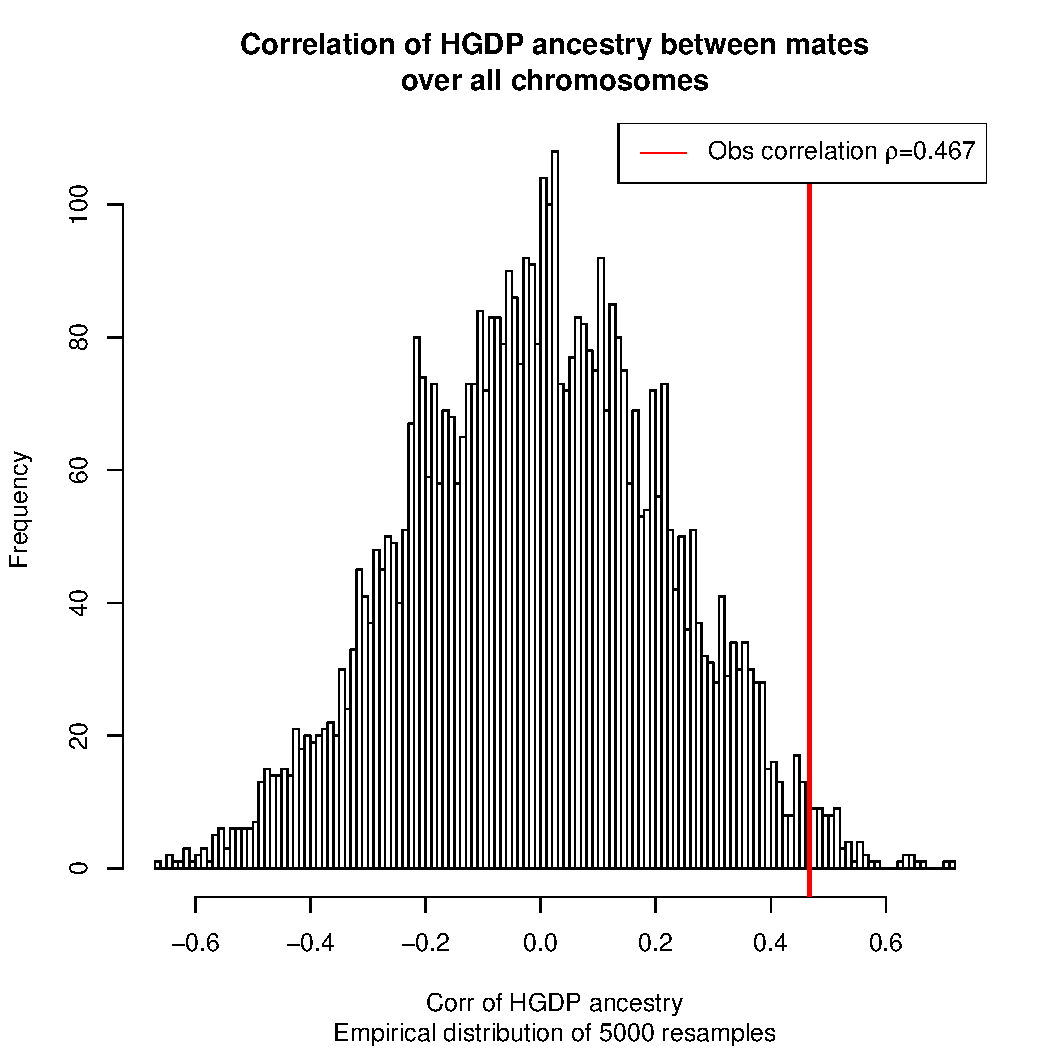
\includegraphics[height=2.75in]{Corr_allChr_mateAncest.png}
\includegraphics[height=2.75in]{Corr_XChr_mateAncest.png}
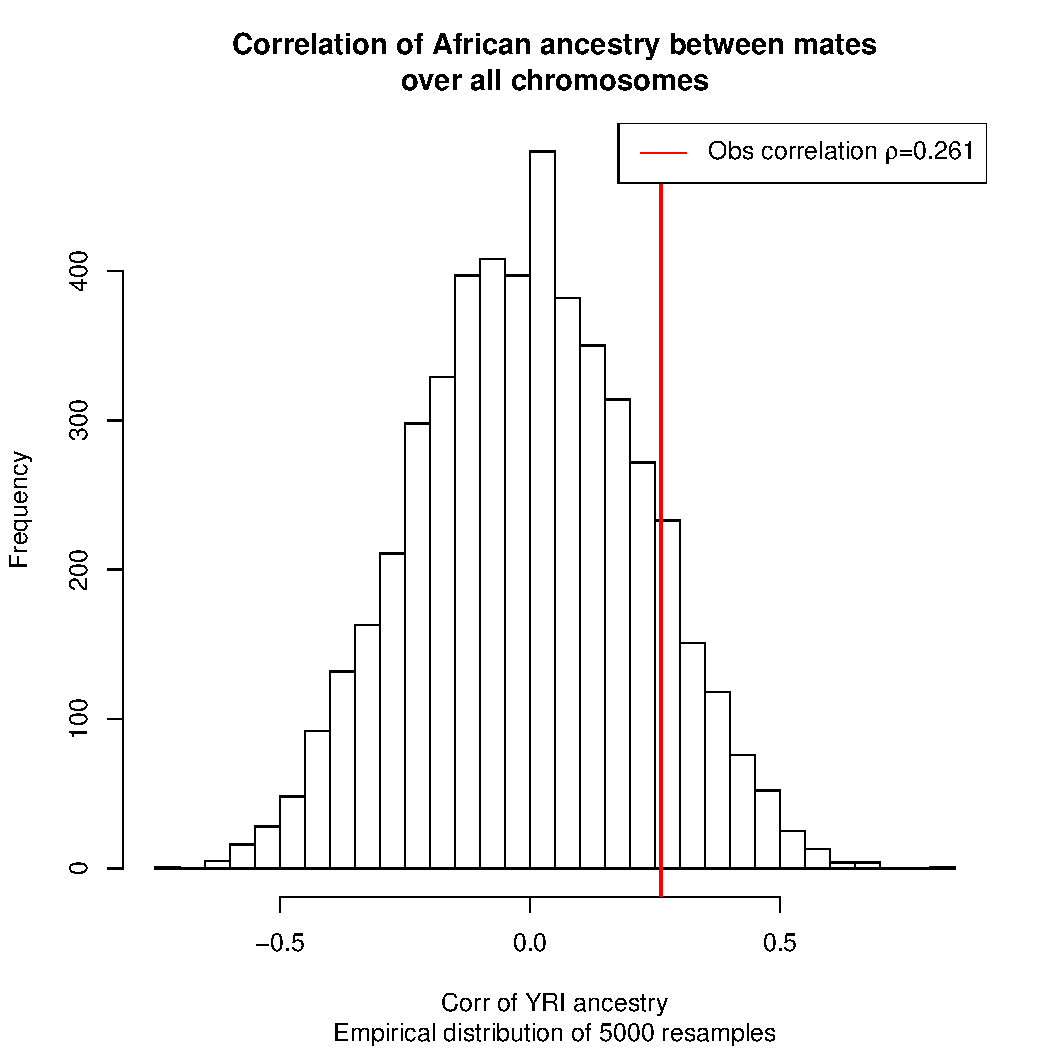
\includegraphics[height=2.75in]{Corr_allChr_mateAncest_YRI.png}
\includegraphics[height=2.75in]{Corr_XChr_mateAncest_YRI.png}
\caption{Correlation of autosomal Native American ancestry, X chromosome Native American ancestry, autosomal African ancestry and X chromosome African ancestry, among 5,000 randomly sampled mate pairs from the 24 MXL mates.
The observed correlation for each case is shown in red.}
\label{fig:hists}
\end{figure}

\begin{table}[ht]
\begin{center}
\begin{tabular}{r|lll|lll}
\hline
&\multicolumn{3}{c|}{X chromosome}&\multicolumn{3}{|c}{Autosomal}\\
statistic& African & Native Am &European& African & Native Am&European \\ \hline
mean & -2.30e-05 &-6.70e-04 &-3.62e-05&-0.003 & -0.005 &6.94e-04\\
SD & 0.21 &0.21 &0.21&0.21 & 0.21&0.21 \\
empirical p-value &0.1826 &  0.0084 &0.0196& 0.1052 & 0.0074 &0.0056 \\
\end{tabular} \end{center} 
\caption{Mean, standard deviation and empirical p-value calculations from 5,000 bootstrap samples shown in Figure~\ref{fig:hists}, for autosomal and X chromosome Native American and African ancestry.}
\end{table}
\end{document}


